\documentclass[12pt,a4paper]{article}
\usepackage[top=0.8in, bottom=0.8in, left=0.8in,right=0.80in]{geometry}
\usepackage[pdftex]{graphicx}
\usepackage[utf8x]{inputenc}
\usepackage{ucs}
\usepackage{natbib}
%\usepackage{float}
\usepackage{hyperref}
\usepackage{pslatex}
\usepackage{tikz}
\usetikzlibrary{intersections,automata,arrows,positioning,calc,shapes.gates.logic.US,trees,positioning,arrows}
\usepackage{rotating}
\usepackage{amsmath}
\usepackage{amssymb}
\setcounter{MaxMatrixCols}{20}
\usepackage{pgfplots}
\pgfplotsset{width=17cm,compat=1.9}
\usepackage{verbatim}
\usepackage{multirow}
%\usepackage{array}
\usepackage{setspace}
\usepackage{enumerate}
%\usepackage{longtable}
%\usepackage[font=small,labelfont=bf]{caption}
%\def\figurename{Figure }
%\usepackage{listings}
\usepackage{color, colortbl}
\usepackage{amsfonts}
\usepackage[T1]{fontenc}
%\usepackage{mathptmx}
\setlength{\parindent}{0pt}
\setlength{\parskip}{5pt}
%\usepackage{lmodern}
%\renewcommand*\familydefault{\sfdefault}

\usepackage{mdframed}

\usepackage{fancyhdr}
\pagestyle{fancy}
\fancyhf{}
\setlength{\headheight}{15pt}
\fancyhead[OR]{\thepage}
\fancyhead[OL]{\nouppercase \leftmark}
\setlength{\parindent}{0pt}
\setlength{\parskip}{5pt}





\usepackage{calc}
\usepackage{array}
\usepackage{tabu}
\usepackage{longtable}
%\usepackage{fontspec}
\usepackage{amsthm}
\usepackage{thmtools}


%Change to alphanumeric section labeling
\def\thesection{\alph{section}}

\begin{document}


\definecolor{TMgreen}{RGB}{14, 191, 48}
\definecolor{TMorange}{RGB}{243, 126, 25}
\definecolor{TMred}{RGB}{230, 6, 85}
\definecolor{TMcodeBackground}{RGB}{224, 224, 224}
\definecolor{TMcodeFrame}{RGB}{109, 108, 109}
\definecolor{TMtableHead}{RGB}{230, 6, 85}
\definecolor{TMtableRowTwo}{RGB}{230, 230, 230}
\definecolor{TMtableRowOne}{RGB}{240, 240, 240}
\definecolor{TMemphasis}{RGB}{165, 32, 23}
\definecolor{TMwarning}{RGB}{250, 175, 52}
\definecolor{TMcritical}{RGB}{229, 0, 72}
\definecolor{TMnormal}{RGB}{54, 160, 220}
\definecolor{TMbulletinBackground}{RGB}{224, 224, 224}
\definecolor{TMtheorem}{RGB}{14, 191, 48}


\newmdenv[
        skipabove=4mm,
        skipbelow=1mm,
        innertopmargin=1mm,
        innerbottommargin=1mm,
        innerleftmargin=0mm,
        innerrightmargin=0pt,
        rightline=false,
        topline=false,
        bottomline=false,
        linewidth=1mm,
%        frametitlefont={\sffamily\bfseries},
        frametitlefont={\bfseries},
        backgroundcolor=TMbulletinBackground]{TMbulletinBase}
\newmdenv[default, linewidth=0pt, backgroundcolor=TMbulletinBackground]{TMbulletinContent}


\mdfdefinestyle{normal}{linecolor=TMnormal}
\mdfdefinestyle{warning}{linecolor=TMwarning}
\mdfdefinestyle{critical}{linecolor=TMcritical}

\newcommand{\TMbulletinTitleContent}[2]{
    \hspace*{2mm}\begin{minipage}{0.75cm}
        \includegraphics[width=\linewidth]{#1}
    \end{minipage}\hspace*{1mm}\begin{minipage}{\textwidth-1.05cm}
            #2
    \end{minipage}
}

\newenvironment{TMbulletin}[2]{
    \begin{TMbulletinBase}[style=#1, frametitle=\TMbulletinTitleContent{icons/#1.png}{#2}]
    \vspace*{1mm}
    \begin{TMbulletinContent}
}
{
    \end{TMbulletinContent}
    \end{TMbulletinBase}
}



\newcommand{\tableCaption}{}
\mdfdefinestyle{TMstyleTable}{
            skipabove=4mm,
            skipbelow=0mm,
            %remove borders
            rightline=false,
            topline=false,
            bottomline=false,
            linewidth=1mm,
            %margins
            innertopmargin=0mm,
            innerleftmargin=0mm,
            innerbottommargin=0mm,
            innerrightmargin=0pt,
            backgroundcolor=TMcodeBackground,
            linecolor=TMtableHead,
}
\everyrow{\tabucline[.4mm white]{}}
\tabulinesep=^3mm_2mm
\taburowcolors[2] 2{TMtableRowOne .. TMtableRowTwo}
\newenvironment{TMtable}[3]
{
    \renewcommand{\tableCaption}{#3}
    \begin{table}[#2]
    \begin{mdframed}[style=TMstyleTable]
    \begin{tabu} to \textwidth{#1}
%        \rowfont{\bfseries\sffamily\leavevmode\color{white}}
        \rowfont{\bfseries\leavevmode\color{white}}
        \rowcolor{TMtableHead!}
}
{
    \end{tabu}
    \end{mdframed}
    \caption{\tableCaption}
    \end{table}
}

\begin{center}
\thispagestyle{empty}
\rule{\textwidth}{1pt}\vspace{0.4cm}
\LARGE{\textbf{TMA4275\\Obligatory Exercise 1}}
\rule{\textwidth}{1pt}
\vspace{5cm}
\Large{\textbf{\\Submitted by\\}}
%\Large{\textbf{\\NTNU Trondheim\\}}
\vspace{0.3cm}
%\Large{\textbf{\\by}}\\[0.3cm]
\Large{100XX\\100XX}\\
\vspace{4.5cm}
\includegraphics[scale=1.5]{project/images/ntnulogo.pdf}\\
\vspace{2cm}
\large{\textbf{\\20.2.2016}}\\[0.5cm]
\end{center}
\newpage
\newpage
\pagenumbering{roman}
\tableofcontents
\newpage
%\listoftables
%\newpage
%\listoffigures
%\newpage
\pagenumbering{arabic}
\section{Kaplan-Meier}
\textit{Use MINITAB to estimate and to draw in the same graph the KaplanMeier estimates $\hat{R}_1 (t)$ and $\hat{R}_2 (t)$.\\
Also let the MINITAB output contain the corresponding 95\% confidence curves.\\
Find and compare the estimated median, lower and upper quartiles of the two distributions.\\
What are the definitions and interpretations of these quantities?\\
How can they be read off from the curves?}
\begin{center}
\line(1,0){250}
\end{center}
la bla here

\newpage
\section{Null Hypothesis}
\textit{Explain how one may use the logrank test to test the null hypothesis that patients with the two tumour types have the same survival distributions.\\
Use the version of the test considered in Slides 6, p. 44-50, and do the necessary calculations for lifetimes up to (and including) 15.\\
It can be shown (you need not do it) that the total number of expected deaths for type 1 is 22.48 and for type 2 is 19.52.\\
Use this to calculate the test statistic of the logrank test, and perform the test with significance level 5\%.\\
What is the lowest significance level that will lead to rejection of the null hypothesis, i.e., what is the p-value?}
\begin{center}
\line(1,0){250}
\end{center}
la bla here


\newpage
\section{Nelson-Aalen}
\textit{First, compute “by hand” the estimates $\hat{Z}_1 (t)$ for $t \le 38$.\\
Then use the MINITAB macro for Nelson-plot to calculate and to graph the complete Nelson-Aalen plot for $T_1$.\\
Does the plot give any indication regarding the hazard function $z_1 (t)$? Explain.}
\begin{center}
\line(1,0){250}
\end{center}
la bla here

%\newpage
%\section{Question 3: Markov possibility}
\textit{We try to model the	same system with a Markov process. Can we take into account all the events described in the table below?}	
 \begin{center}
\line(1,0){250}
\end{center}
One of the big advantages of using the markov state diagram approach is its versatility. Virtually every system can be modelled with it. The size and complexity can increase into a level in which calculation by hand is not feasable. However, it is then still a good method to illustrate a system and its possible states and transitions, without using it for further calculations. An exemplary markov state diagram of such purpose can be found in figure \ref{fig:markov_complex}.

\begin{figure}[!ht]
\centering
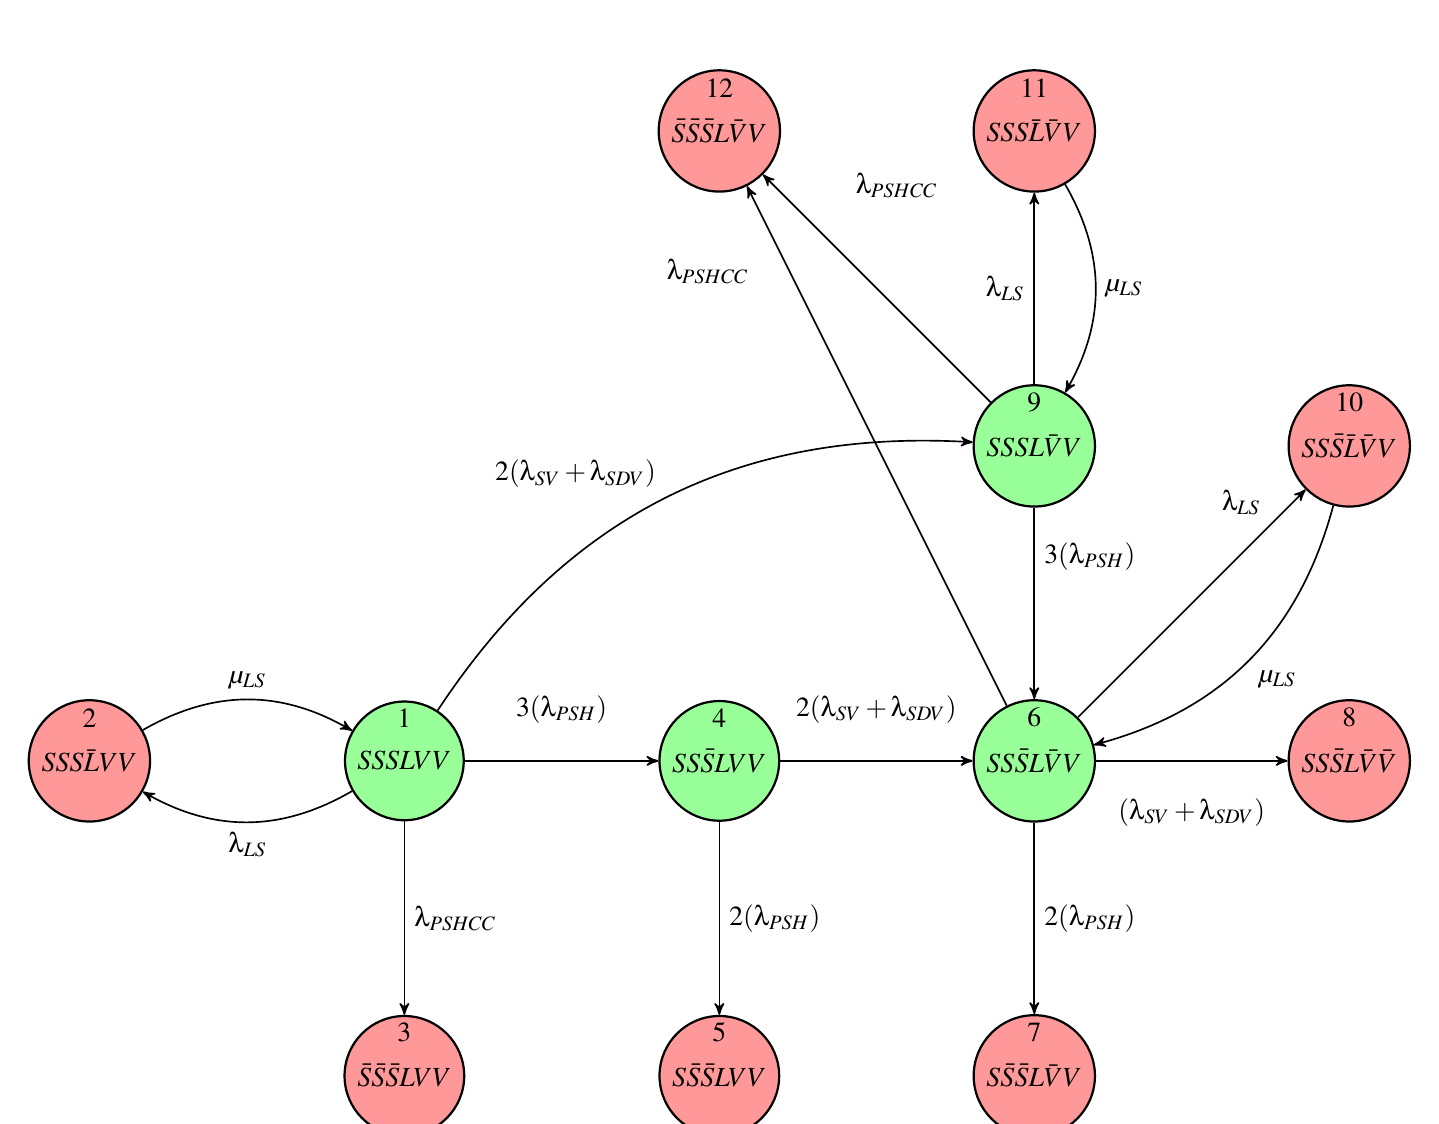
\begin{tikzpicture}[->, >=stealth', auto, semithick, node distance=4cm]
\tikzstyle{every state}=[fill=green!40,draw=black,thick,text=black,scale=1]
\tikzstyle{fail}=[circle,fill=red!40,draw=black,thick,text=black,scale=1]
\node[state]    (1)                     {$SSSLVV$};
\node[fail]     (L)[left of=1]          {$SSS\bar{L}VV$};
\node[fail]    (CC)[below of=1]        {$\bar{S}\bar{S}\bar{S}LVV$};
\node[state]    (S)[right of=1]         {$SS\bar{S}LVV$};
\node[fail]    (SS)[below of=S]        {$S\bar{S}\bar{S}LVV$};
\node[state]    (SV)[right of=S]       {$SS\bar{S}L\bar{V}V$};
\node[fail]    (SSV)[below of=SV]      {$S\bar{S}\bar{S}L\bar{V}V$};
\node[state]    (V)[above of=SV]        {$SSSL\bar{V}V$};
\node[fail]    (LV)[above of=V]        {$SSS\bar{L}\bar{V}V$};
\node[fail]    (VCC)[left of=LV]       {$\bar{S}\bar{S}\bar{S}L\bar{V}V$};
\node[fail]    (SVV)[right of=SV]      {$SS\bar{S}L\bar{V}\bar{V}$};
\node[fail]    (SLV)[above of=SVV]     {$SS\bar{S}\bar{L}\bar{V}V$};
\path
(1)     edge[bend left, below]    node{$\lambda_{LS}$}               (L)
        edge[]              node{$\lambda_{PSHCC}$}          (CC)
        edge[]              node[yshift=0.35cm]{$3(\lambda_{PSH})$}         (S)
        edge[bend left]     node{$2(\lambda_{SV}+\lambda_{SDV})$}(V)
        node[above=0.3cm]{1}
%
(S)     edge[]              node{$2(\lambda_{PSH})$}        (SS)
        edge[]              node[yshift=0.35cm]{$2(\lambda_{SV}+\lambda_{SDV})$}(SV)
        node[above=0.3cm]{4}
%        
(SV)    edge[]              node{$2(\lambda_{PSH})$}        (SSV)
        edge[]              node[yshift=2.5cm][xshift=-1.5cm]{$\lambda_{PSHCC}$}      (VCC)
        edge[below]         node[yshift=-0.35cm]{$(\lambda_{SV}+\lambda_{SDV})$}(SVV)
        edge[]              node[yshift=1cm][xshift=1cm]{$\lambda_{LS}$}(SLV)
        node[above=0.3cm]{6}
%
(V)     edge[]              node[yshift=0.6cm]{$3(\lambda_{PSH})$}    (SV)
        edge[]              node[yshift=1.6cm][xshift=0.9cm]{$\lambda_{PSHCC}$}    (VCC)
        edge[]              node{$\lambda_{LS}$}(LV)
        node[above=0.3cm]{9}
%
(L)     edge[bend left, above]    node{$\mu_{LS}$}               (1)
        node[above=0.3cm]{2}
%
(LV)    edge[bend left]    node{$\mu_{LS}$}               (V)
        node[above=0.3cm]{11}
%
(CC)    node[above=0.3cm]{3}
(SS)    node[above=0.3cm]{5}
(SSV)   node[above=0.3cm]{7}
(SVV)   node[above=0.3cm]{8}
(VCC)   node[above=0.3cm]{12}
%
(SLV)   edge[bend left]    node{$\mu_{LS}$}               (SV)
        node[above=0.3cm]{10};
%\node[above=0.3cm] (1){\small{1}};
%\node[yshift=-3.5cm, above of=1] (L){\small{1}};
%\node[yshift=-3.5cm, above of=L] (L){\small{2}};
%\node[above=0.5cm] (L){\small{2}};
%    edge[]             node{$\lambda_{PSHCC}$}      (E)
%(B) edge[]             node{$2\lambda_{PSH}$}           (C)
%    edge[]             node{$2(\lambda_V+\lambda_{DV})$}   (D)
%(C) edge               node{$1$}           (D)
%(D) %edge[loop right]    node{$(1-q)^2$}     (D)
    %edge[bend right,right]    node{$q(1-q)$}      (B)
    %edge[bend left]     node{$q(1-q)$}      (C)
%    edge[bend left,above]     node{$\mu_L$}         (A);
%\draw[red] ($(D)+(-1.5,0)$) ellipse (2cm and 3.5cm)node[yshift=3cm]{Patch H};
%;
\end{tikzpicture}
\caption{Complex markov state diagram }\label{fig:markov_complex}
\end{figure}

Each state is given in the notation $SSSLVV$. The three $S$ indicate the condition of the pressure sensors, the $L$ gives information about the functionality of the logic solver and the $VV$ part represents the two valve sets. Working states are indicated by green color and failed states by red color.

This expanded diagram allows to illustrate the various changes of partial failed states into other partial failed states and subsequently fully failed states.
As an example, the system can be in a functioning state with one pressure sensor failed and transit into another functioning state with one valve set failed.
This diagram also includes the possible repair of the logic solver.

\newpage

% Please add the following required packages to your document preamble:
% \usepackage{multirow}



%$\begin{bmatrix}
%  \scriptscriptstyle{-(\lambda_L+\lambda_{PSHCC}+3\lambda_{PSH}+2(\lambda_{SV}+\lambda_{SDV}))} & \lambda_L & \lambda_{PSHCC} & 3\lambda_{PSH} & 0 & 0 & 0 & 0 & \scriptscriptstyle{2(\lambda_{SV}+\lambda_{SDV})} & 0 & 0 & 0 \\
%  \mu_L & -\mu_L & 0 & 0 & 0 &0 & 0 & 0 & 0 & 0 & 0& 0\\
%    0 & 0 & 0 & 0 & 0 &0 & 0 & 0 & 0 & 0 & 0& 0 \\
%    0 & 0 & 0 & 0 & 0 &0 & 0 & 0 & 0 & 0 & 0& 0 \\
%    1 & 2 & 3 & \scriptscriptstyle{-(2\lambda_{PSH}+2(\lambda_{SV}+\lambda_{SDV})) & 2\lambda_{PSH}} &\scriptscriptstyle{2(\lambda_{SV}+\lambda_{SDV})} & 7 & 8 & 9 & 10 & 11& 12 \\
%    1 & 2 & 3 & 4 & 5 &6 & 7 & 8 & 9 & 10 & 11& 12 \\
%    1 & 2 & 3 & 4 & 5 &6 & 7 & 8 & 9 & 10 & 11& 12 \\
%    1 & 2 & 3 & 4 & 5 &6 & 7 & 8 & 9 & 10 & 11& 12 \\
%    1 & 2 & 3 & 4 & 5 &6 & 7 & 8 & 9 & 10 & 11& 12 \\
%    1 & 2 & 3 & 4 & 5 &6 & 7 & 8 & 9 & 10 & 11& 12 \\
%    1 & 2 & 3 & 4 & 5 &6 & 7 & 8 & 9 & 10 & 11& 12 \\
%    1 & 2 & 3 & 4 & 5 &6 & 7 & 8 & 9 & 10 & 11& 12 \\
% \end{bmatrix}$
 

%  $\begin{bmatrix}
% 1 & 2 & 3 & 4 & 5 &6 & 7 & 8 & 9 & 10 & 11& 12 \\
%  1 & 2 & 3 & 4 & 5 &6 & 7 & 8 & 9 & 10 & 11& 12
% \end{bmatrix}$
%\newpage
%\section{Question 4: State diagram}
\textit{Give the state transition diagram related to this system, without any maintenance	action.}
\begin{center}
\line(1,0){250}
\end{center}
Figure \ref{fig:markov_simple} introduces a simplified markov state diagram. It is derived from figure \ref{fig:markov_complex} but lacks many transitions. The number of possible states is reduced from 12 to 4, no maintenance is possible. The fail states have been reduced to "Failure of Valves", "Failure of Sensors" and "Failure of Logic Solver" - with the respective combined failure rates $\lambda_V$, $\lambda_S$ and $\lambda_L$. No transition between partly functioning states is possible.

\begin{figure}[!ht]
\centering
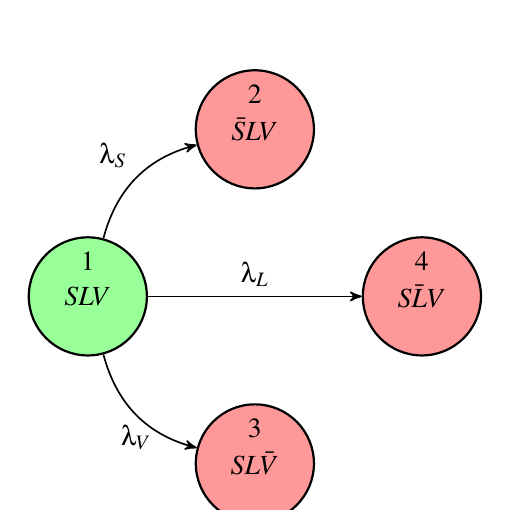
\begin{tikzpicture}[->, >=stealth', auto, semithick, node distance=3cm]
\tikzstyle{every state}=[fill=green!40,draw=black,thick,text=black,scale=1,minimum width=1.5cm]
\tikzstyle{fail}=[circle,fill=red!40,draw=black,thick,text=black,scale=1,minimum width=1.5cm]
\node[state]    (A)                     {$SLV$};
\node[fail]    (B)[above right of=A]   {$\bar{S}LV$};
\node[fail]    (C)[below right of=A]   {$SL\bar{V}$};
\node[fail]    (D)[below right of=B]   {$S\bar{L}V$};
\path
(A) edge[bend left]     node{$\lambda_S$}     (B)
    edge[]      node{$\lambda_L$}      (D)
    edge[bend right, below]    node{$\lambda_V$}      (C)
    node[above=0.2cm]{1}
(B) node[above=0.2cm]{2}
(C) node[above=0.2cm]{3}
(D) node[above=0.2cm]{4}
%(B) edge                node{$1$}           (D)
%(C) edge                node{$1$}           (D)
%(D) %edge[loop right]    node{$(1-q)^2$}     (D)
    %edge[bend right,right]    node{$q(1-q)$}      (B)
    %edge[bend left]     node{$q(1-q)$}      (C)
%    edge[bend left,above]     node{$\mu_L$}         (A);
%\draw[red] ($(D)+(-1.5,0)$) ellipse (2cm and 3.5cm)node[yshift=3cm]{Patch H};
;
\end{tikzpicture}
\caption{Simple markov state diagram without maintenance}\label{fig:markov_simple}
\end{figure}
%\newpage
%\section{Question 5: Reliability}
\textit{Calculate the reliability of the system at the steady state.}
\begin{center}
\line(1,0){250}
\end{center}
The matrix formula
$\begin{bmatrix}
P1 & P2 & P3 & P4
\end{bmatrix}$
$\times$
$\begin{bmatrix}
 -(\lambda_S+\lambda_V+\lambda_L) & \lambda_S & \lambda_V & \lambda_L\\
 0 & 0 & 0 & 0\\
 0 & 0 & 0 & 0\\
 0 & 0 & 0 & 0\\
 \end{bmatrix}$
 $= 0$
 
results in following 5 equations, including the boundary condition V:


\begin{table}[!ht]
\centering
\label{tab:equations}
\begin{tabular}{ll}
I   & $-P1\times(\lambda_S+\lambda_V+\lambda_L) = 0$ \\
II  & $P1\times\lambda_S = 0$ \\
III & $P1\times\lambda_V = 0$ \\
IV  & $P1\times\lambda_L = 0$ \\
V   & $P1+P2+P3+P4 = 1$ 
\end{tabular}
\end{table}

From above equations the steady state reliability is $0$. This is independent of the actual numerical values for the various failure rates. This conclusion is trivial, as from the logical approach this result can be achieved easier: A system which only includes failure rates, but no repair rates, will eventually reach (and be kept in) a failed state if time steps into infinity.
%\newpage
%\section{Question 6: Maintenance Strategy}
\textit{Only the logic solver is repairable	as explained in	the last slide with	the GLM distribution. This is purely corrective	maintenance. Do you think you could recommend preventive maintenance strategies in addition to the corrective one? Which kind of preventive maintenance strategies? Give a methodology to evaluate the performance of the proposed preventive maintenance strategies.}
\begin{center}
\line(1,0){250}
\end{center}
In the current system description the Logic Solver is the only component given which is repairable. Furthermore, only corrective maintenance is intended.

Several approaches can be taken to change the maintenance structure.

\textbf{Stick to corrective maintenance:}
If the parameters of the repair process are optimal (Spare unit on stock, quick exchange possible, low downtime, low value of spare item) it can be economical beneficial to continue performing only corrective maintenance in case of a failure.

\textbf{Change to clock-based maintenance:}
Depending on the maintenance strategy and operation of the rest of the system, clock-based maintenance can be an option. This is the case, if other parts of the system already undergo clock-based maintenance and thus the maintenance for the Logic Solver can be added to it in a similar way.

\textbf{Change to age-based maintenance:}
The age-based maintenance is another approach which, if implemented correctly, can reduce overall lifecycle costs and increase the overall system performance. It is required to have the possibility to log the operation time of the Logic Solver. 

\textbf{Change to condition-based maintenance:}
The most advanced maintenance system is based on the condition of the item. Rather than changing it based on time in use or operation hours, the actual condition and functionality of the device is monitored. For items like Logic Solvers this can be implemented by having a periodic self-check with a feedback routine to inform personnel about an upcoming defect.
Implementing such a system is increasing the fixed operation costs and may create investment costs. Additionally condition based maintenance requires trained personnel, which may increase costs as well.

\textbf{Evaluating different methods:}
To evaluate the best maintenance method, it is necessary to gather information about the system beforehand:

\begin{itemize}
\item Costs for corrective maintenance
\item Costs for preventive maintenance
\item Costs for implementing clock/age/condition-based maintenance
\item Downtime cost and duration in case of corrective maintenance
\item Downtime cost and duration in case of preventive maintenance
\item Effectiveness of preventive maintenance (revert back to as-new state possible?)
\item Current maintenance approach at the rest of the system for possible synchronisation
\item Failure distribution model for item in scope (Exponential in case of Logic Solver)
\end{itemize}

After assessing the information it is possible to create mathematical formulas expressing the maintenance costs depending on the time. This numerical approach allows to plot a comparative array of graphs. A qualitative result is quickly found by that, and additionally a quantitative evaluation can be done afterwards to derive the optimal parameters for the selected maintenance system.
\newpage
\section{Showing boxes}

\begin{TMbulletin}{warning}{Test Warning}
    Malesuada ligula sociosqu faucibus a venenatis ridiculus ante scelerisque
    dui nulla leo platea condimentum vestibulum a aliquam. Libero litora
    ullamcorper justo diam nascetur parturient enim ad enim a nullam elit metus
    himenaeos dictum hac semper at adipiscing ac tempor laoreet hac parturient
    elementum.
\end{TMbulletin}


\begin{TMbulletin}{normal}{Test Normal}
    Parturient metus senectus ut dis ante sit a id dis urna imperdiet neque
    fermentum vehicula consectetur varius feugiat tempus himenaeos ad nisi
    curabitur.Ultricies dis parturient nulla vel vestibulum sodales fames
    faucibus quis.
\end{TMbulletin}


\begin{TMbulletin}{critical}{Test Critical}
    Iaculis ad ac vivamus scelerisque a ultrices a volutpat eget porta non mus
    scelerisque convallis dictumst.Condimentum velit consequat fringilla.
\end{TMbulletin}


\begin{TMtable}{X X X X}{ht!}{Description of Table} 
        N & Result & Absolute error & Time [sec]\\
        5& 0.1734& 0.0193& 0.0011\\ 
        10& 0.1864& 0.0063& 0.0675\\ 
        15& 0.1897& 0.0030& 0.8190\\
        20& 0.1910& 0.0016& 4.3892\\ 
\end{TMtable}
\newpage
\bibliographystyle{agsm}
\addcontentsline{toc}{section}{References}
\setstretch{1}
\bibliography{project/literature.bib}
\newpage
\end{document}